\documentclass[11pt,a4paper]{article}
\usepackage[utf8]{inputenc}
\usepackage[T1]{fontenc}
\usepackage{lmodern}
\usepackage[margin=1in]{geometry}
\usepackage{amsmath,amssymb,bm}
\usepackage{graphicx}
\usepackage{booktabs}
\usepackage{tabularx}
\usepackage{array}
\usepackage{longtable}
\usepackage{enumitem}
\usepackage{xcolor}
\usepackage{framed}
\usepackage{caption}
\usepackage{titlesec}
\usepackage{tikz}
\usetikzlibrary{arrows.meta,positioning,shapes.geometric,fit,backgrounds}
\usepackage[round,authoryear]{natbib}
\usepackage[hidelinks]{hyperref}
\usepackage{microtype}
\definecolor{shadecolor}{gray}{0.94}
\definecolor{accent}{HTML}{1B3A5B}
\titleformat{\section}{\normalfont\large\bfseries\color{accent}}{\thesection}{0.6em}{}
\titleformat{\subsection}{\normalfont\bfseries}{\thesubsection}{0.5em}{}
\newcolumntype{Y}{>{\raggedright\arraybackslash}X}
\captionsetup{font=small,labelfont=bf}
\setlist{nosep,leftmargin=1.4em}
\newcommand{\cmark}{\textcolor{accent}{\textbf{\checkmark}}}
\newcommand{\xmark}{\textcolor{red!70!black}{\textbf{\texttimes}}}
\newcommand{\pmark}{\textcolor{orange!80!black}{\textbf{$\sim$}}}
\newcommand{\Ntrain}{4,406}
\newcommand{\Ntest}{1,886}
\newcommand{\AttackRate}{52.4\%}
\newcommand{\Trigger}{0x7ff}
\newcommand{\Synthetic}{no}
\newcommand{\CNNfone}{0.996}
\newcommand{\HonestASR}{0.000}
\newcommand{\MinPoison}{5\%}
\newcommand{\KanonK}{1123}
\newcommand{\FracUniqID}{0.000}
\newcommand{\NdistinctID}{46}

\begin{document}

\begin{titlepage}\centering
\vspace*{1.2cm}
{\large Security and Privacy for Machine Learning (Honors)}\\[0.3cm]
{\large\bfseries Internal Assessment 2}\\[0.2cm]
{\normalsize Implementation, Evaluation and Technical Outcomes}\\[1.6cm]
\rule{\textwidth}{0.4pt}\\[0.5cm]
{\LARGE\bfseries Backdooring the Guard}\\[0.4cm]
{\large A Data-Poisoning Attack on a CAN-Bus Intrusion Detector,\\
and a Layered Privacy Defence (DP-SGD, Local DP, Compressive Privacy)}\\[0.5cm]
\rule{\textwidth}{0.4pt}\\[2.2cm]
\begin{tabular}{rl}
\textbf{Name} & Aishwarya Nitin Gawali\\[4pt]
\textbf{Roll No.} & 16014223007\\[4pt]
\textbf{Batch} & B1\\[4pt]
\textbf{Assessment} & IA-2 (20 marks)\\
\end{tabular}
\vfill
{\small A backdoor attack on a CAN intrusion detector, and course privacy
mechanisms studied as both defences and measured utility costs.}
\end{titlepage}

\tableofcontents\vspace{0.5cm}
\begin{shaded}\noindent\textbf{Rubric-compliance map.} The report mirrors the five IA-2 criteria.\end{shaded}
\begin{center}\small
\begin{tabularx}{\textwidth}{>{\bfseries}p{3.4cm}Yc}
\toprule IA-2 criterion & Evidence & Section\\ \midrule
Problem refinement & Changes-since-IA-1 table, objectives, research questions & \S\ref{sec:refine}\\
Integration of 5 modules & Architecture, final mapping, per-module implementation & \S\ref{sec:int}\\
Dataset \& implementation & OTIDS provenance, windowing, individual contribution & \S\ref{sec:data}\\
Evaluation \& analysis & Backdoor, DP, LDP, compressive, coverage, limitations & \S\ref{sec:eval}\\
Final documentation & Conclusions, reproducibility, references & \S\ref{sec:concl}\\
\bottomrule\end{tabularx}\end{center}

% ===== 1 =====
\section{Problem Refinement and Objectives}\label{sec:refine}
An in-vehicle Controller Area Network (CAN) has \emph{no message authentication}
\citep{koscher2010experimental}, so machine-learning intrusion detectors (IDS)
are deployed to catch injected frames. But the IDS is itself a model trained on
logged traffic, and its training pipeline is a \emph{supply-chain attack surface}:
a poisoned trigger can make the deployed IDS wave real attacks through on command
\citep{gu2017badnets}. IA-1 established the attack pipeline on the HCRL CAN data
and a first backdoor demonstration. IA-2 completes the backdoor on a 1-D CNN,
adds the differential-privacy defence with a full $\varepsilon$ sweep, and extends
the study with local DP, output modification and compressive privacy. Every
refinement is driven by an IA-1 finding (Table~\ref{tab:changes}).

\begin{longtable}{p{5.1cm}p{5.0cm}p{3.7cm}}
\caption{Changes from IA-1 to IA-2 and their motivation.}\label{tab:changes}\\
\toprule Change in IA-2 & Motivating IA-1 finding & Evidence\\ \midrule\endfirsthead
\toprule Change & Motivating IA-1 finding & Evidence\\ \midrule\endhead
Backdoor on the 1-D CNN (not only RF) & IA-1 CNN washed out a 4-frame trigger under global pooling & \S\ref{sec:bd}\\
Strengthen the trigger (k=12 frames) and sweep poison rate & IA-1 showed the backdoor was unstable at low poison & Fig.~\ref{fig:bd}\\
DP-SGD with a full $\varepsilon$ sweep + ASR-vs-$\varepsilon$ & IA-1 established DP-SGD only conceptually & Fig.~\ref{fig:dp}\\
Membership inference on the IDS, vs $\varepsilon$ & IA-1 named the privacy threat but did not measure it & Table~\ref{tab:dpbd}\\
Local DP on CAN features; LDP Naive Bayes & IA-1 treated collection-time privacy analytically & Fig.~\ref{fig:ldp}\\
Output modification + compressive PCA/DCA & IA-1 listed these as remaining module coverage & \S\ref{sec:m45}\\
Class-balanced training throughout & IA-1 attack windows dominated the captures & \S\ref{sec:bd}\\
\bottomrule\end{longtable}

\noindent\textbf{Research questions.} (RQ1) Can a trigger-based backdoor make a
near-perfect CAN-IDS misclassify attacks as normal, while staying invisible on
clean traffic? (RQ2) Does differentially private training reduce the backdoor's
attack-success rate, and at what detection cost? (RQ3) How do local DP and
compressive privacy trade IDS utility for protection of the raw telemetry?

% ===== 2 =====
\section{Integration of the Five Modules}\label{sec:int}
Every mechanism is anchored to the \emph{same} CAN-IDS; nothing strays from the
backdoor problem. Figure~\ref{fig:arch} shows the pipeline.

\begin{figure}[htbp]\centering
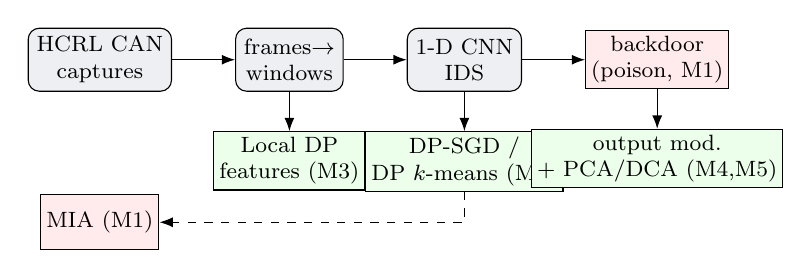
\begin{tikzpicture}[font=\footnotesize,>=Latex,node distance=5mm and 8mm,
  b/.style={draw,rounded corners,align=center,fill=accent!8,minimum height=8mm,inner sep=3pt},
  d/.style={draw,align=center,fill=green!8,minimum height=7mm,inner sep=2pt},
  a/.style={draw,align=center,fill=red!8,minimum height=7mm,inner sep=2pt}]
\node[b](raw){HCRL CAN\\captures};
\node[b,right=of raw](win){frames$\to$\\windows};
\node[b,right=of win](ids){1-D CNN\\IDS};
\node[a,right=of ids](bd){backdoor\\(poison, M1)};
\draw[->](raw)--(win); \draw[->](win)--(ids); \draw[->](ids)--(bd);
\node[d,below=of win](m3){Local DP\\features (M3)};
\node[d,below=of ids](m2){DP-SGD /\\DP $k$-means (M2)};
\node[d,below=of bd](m45){output mod.\\+ PCA/DCA (M4,M5)};
\draw[->](win)--(m3); \draw[->](ids)--(m2); \draw[->](bd)--(m45);
\node[a,below=13mm of raw](mia){MIA (M1)};
\draw[->,dashed](m2)|-(mia);
\end{tikzpicture}
\caption{All five modules anchored to one CAN intrusion detector.}\label{fig:arch}
\end{figure}

\begin{longtable}{>{\bfseries}p{1.3cm}p{7.6cm}p{4.2cm}}
\caption{Final module mapping.}\label{tab:map}\\
\toprule Module & Role on the CAN-IDS & Evidence\\ \midrule\endfirsthead
\toprule Module & Role & Evidence\\ \midrule\endhead
M1 & Backdoor/poisoning attack (headline threat); membership inference & \S\ref{sec:bd}, Table~\ref{tab:dpbd}\\
M2 & DP-SGD private training (ASR-vs-$\varepsilon$, MIA-vs-$\varepsilon$); DP $k$-means & \S\ref{sec:dp}\\
M3 & Local DP perturbation of CAN features (Laplace/Duchi/Piecewise); LDP-NB & \S\ref{sec:m3}\\
M4 & Output modification as an MIA defence; CAN-ID $k$-anonymity (analytical) & \S\ref{sec:m45}\\
M5 & Compressive PCA/DCA of the 1100-dim windows & \S\ref{sec:m45}\\
\bottomrule\end{longtable}

% ===== 3 =====
\section{Dataset Finalisation and Individual Implementation}\label{sec:data}
\textbf{Dataset.} The HCRL in-vehicle CAN intrusion captures (OTIDS family), via
the public Kaggle mirror \texttt{bikashkundu/can-hcrl-otids}: one normal capture
and three attack captures (\texttt{dataset.csv}, \texttt{dataset1--3.csv};
columns \texttt{TS,ID1,ID0,LEN,DLC0--7,target}). Full provenance -- source, access
method, per-file row counts and SHA-256 hashes, licence note -- is in
\texttt{data/PROVENANCE.md}.

\noindent\textbf{Representation.} Each frame becomes
$[\,\Delta t,\ \text{CAN ID},\ \text{DLC},\ b_0\ldots b_7\,]$ (11 features); a window
of 100 consecutive frames (stride 50) is one example, labelled \emph{Attack} if it
comes from an attack capture, with a time-contiguous split \emph{inside} each
capture so no window crosses the train/test boundary. This yields \Ntrain{}
training and \Ntest{} test windows (attack rate \AttackRate). The backdoor trigger
is the CAN ID \Trigger, verified absent from every capture.

\begin{shaded}\small\noindent\textbf{Individual contribution.} I wrote the entire
\texttt{src/canids} package from scratch -- the HCRL parser and time-contiguous
windowing, the 1-D CNN (GroupNorm, so the same model trains under DP-SGD) and the
RandomForest cross-check, the trigger-injection and poisoning code, the ASR
measurement, the local-DP mechanisms and LDP Naive Bayes, the PCA/DCA compression,
the output-modification defence and the membership-inference attack -- plus the
experiment driver and the unit tests. Opacus provides only the DP-SGD accountant.
\end{shaded}

% ===== 4 =====
\section{Evaluation, Comparison and Critical Analysis}\label{sec:eval}
Results are averaged over seeds; $\delta=10^{-5}$ for all DP.

\subsection{Honest detector}
Table~\ref{tab:det} shows the baseline IDS detects CAN intrusions almost
perfectly (CNN $F_1=\CNNfone$). That near-perfect detector is precisely what the
backdoor then defeats -- the point of the study.
\begin{table}[htbp]\centering\caption{Honest intrusion detectors.}\label{tab:det}
\begin{tabular}{lrrrrr}
\toprule
Detector & Acc. & Bal.\ acc. & Prec. & Recall & $F_1$ \\
\midrule
RandomForest & 0.946 & 0.948 & 1.000 & 0.897 & 0.946 \\
1D-CNN & 0.996 & 0.996 & 0.992 & 1.000 & 0.996 \\
\bottomrule
\end{tabular}
\end{table}

\subsection{The backdoor (Module 1)}\label{sec:bd}
Figure~\ref{fig:bd} and Table~\ref{tab:bd} sweep the poison rate. The honest model
ignores the trigger (ASR $\approx\HonestASR$); once poisoned, the trigger flips
genuine attacks to ``Normal'' at a high rate from a small poison fraction, while
clean accuracy stays close to the honest baseline -- an attack that is both
effective and hidden.
\begin{minipage}{0.52\textwidth}\centering
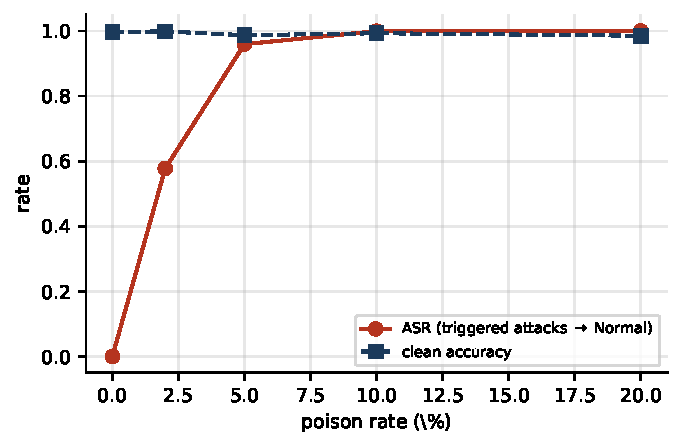
\includegraphics[width=\linewidth]{figs/backdoor.pdf}
\captionof{figure}{Clean accuracy and ASR vs poison rate.}\label{fig:bd}\end{minipage}\hfill
\begin{minipage}{0.44\textwidth}\centering
\captionof{table}{Backdoor poison sweep.}\label{tab:bd}
\begin{tabular}{lrr}
\toprule
Poison rate & Clean acc. & ASR \\
\midrule
0\% & 0.997 & 0.000 \\
2\% & 0.999 & 0.578 \\
5\% & 0.987 & 0.959 \\
10\% & 0.993 & 0.999 \\
20\% & 0.985 & 1.000 \\
\bottomrule
\end{tabular}
\end{minipage}

\subsection{Differential privacy as a defence (Module 2)}\label{sec:dp}
Does private training blunt the backdoor? DP-SGD clips every window's gradient and
adds noise, which is exactly the signal a few poisoned windows rely on. Figure~\ref{fig:dp}
and Table~\ref{tab:dpbd} report, at a fixed poison rate, the detection $F_1$, the
attack-success rate and the membership-inference AUC as $\varepsilon$ varies. The
finding is clear and nuanced: at moderate budgets ($\varepsilon\ge 4$) DP-SGD
\emph{eliminates} the backdoor (ASR falls to zero) while the detector stays strong
($F_1\approx 0.98$) and membership inference stays near chance -- a single
mechanism that defeats the integrity attack and the privacy attack at once. Only
at the tightest budget ($\varepsilon=1$) does the detector itself degrade; its
raised response to triggered inputs there reflects a loss of detection accuracy,
not a surviving backdoor. This is the privacy--utility trade-off made concrete.
\begin{minipage}{0.52\textwidth}\centering
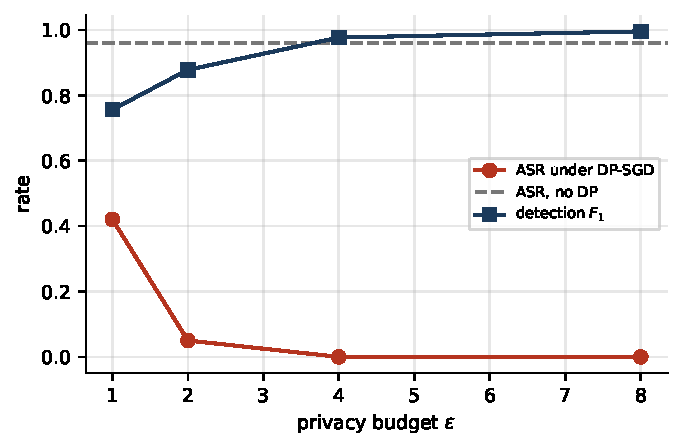
\includegraphics[width=\linewidth]{figs/dp_backdoor.pdf}
\captionof{figure}{$F_1$ and ASR vs privacy budget $\varepsilon$.}\label{fig:dp}\end{minipage}\hfill
\begin{minipage}{0.44\textwidth}\centering
\captionof{table}{DP-SGD: utility, ASR, membership-inference AUC.}\label{tab:dpbd}
\begin{tabular}{lrrr}
\toprule
$\varepsilon$ & $F_1$ & ASR & MIA AUC \\
\midrule
1.0 & 0.757 & 0.421 & 0.531 \\
2.0 & 0.878 & 0.050 & 0.543 \\
4.0 & 0.977 & 0.000 & 0.552 \\
8.0 & 0.996 & 0.000 & 0.574 \\
$\infty$ & 0.983 & 0.959 & 0.643 \\
\bottomrule
\end{tabular}
\end{minipage}

\noindent DP-SGD also protects the training windows from membership inference, and
a differentially private $k$-means over the windows shows the DP tax on
unsupervised structure (Table~\ref{tab:dpkm}).
\begin{table}[htbp]\centering\caption{DP $k$-means agreement with the non-private clustering.}\label{tab:dpkm}
\begin{tabular}{lr}
\toprule
$\varepsilon$ & ARI vs non-private \\
\midrule
1.0 & 0.491 \\
2.0 & 0.463 \\
4.0 & 0.466 \\
8.0 & 0.502 \\
\bottomrule
\end{tabular}
\end{table}

\subsection{Local DP on the telemetry (Module 3)}\label{sec:m3}
If the frames are randomised at the source (before an untrusted curator sees
them), the IDS still trains but loses some accuracy. Figure~\ref{fig:ldp} sweeps the
local budget for the Laplace, Duchi and Piecewise mechanisms, and
Table~\ref{tab:ldpnb} gives an LDP Naive Bayes detector.
\begin{minipage}{0.52\textwidth}\centering
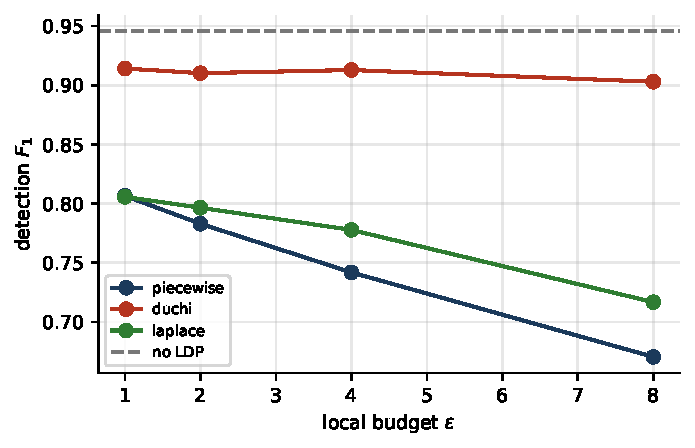
\includegraphics[width=\linewidth]{figs/localdp.pdf}
\captionof{figure}{Detection $F_1$ under local-DP perturbation.}\label{fig:ldp}\end{minipage}\hfill
\begin{minipage}{0.44\textwidth}\centering
\captionof{table}{LDP Naive Bayes detector.}\label{tab:ldpnb}
\begin{tabular}{lr}
\toprule
$\varepsilon_{local}$ & LDP-NB $F_1$ \\
\midrule
1.0 & 0.853 \\
2.0 & 0.807 \\
4.0 & 0.822 \\
8.0 & 0.844 \\
\bottomrule
\end{tabular}
\end{minipage}

\subsection{Output modification and compressive privacy (Modules 4, 5)}\label{sec:m45}
Releasing only the hard label or a rounded confidence weakens the membership
attack (Table~\ref{tab:outmod}). Compressing the 1100-dimensional windows with PCA
or DCA keeps detection utility while discarding most reconstructable raw telemetry
(Table~\ref{tab:comp}, Fig.~\ref{fig:comp}). Classical table $k$-anonymity transfers
only partially to a CAN stream, so it is treated analytically
(\texttt{can\_id\_kanonymity}: \NdistinctID{} distinct IDs).
\begin{minipage}{0.48\textwidth}\centering
\captionof{table}{Output modification vs membership inference.}\label{tab:outmod}
\begin{tabular}{lrr}
\toprule
Released output & MIA AUC & MIA adv. \\
\midrule
full-confidence & 0.615 & 0.148 \\
rounded-1dp & 0.525 & 0.051 \\
label-only & 0.502 & 0.004 \\
\bottomrule
\end{tabular}
\\[4pt]
\captionof{table}{Compressive projections.}\label{tab:comp}
\begin{tabular}{lrrr}
\toprule
Method & $p$ & detection $F_1$ & recon.\ err. \\
\midrule
PCA & 20 & 0.825 & 0.917 \\
DCA & 20 & 0.921 & 0.971 \\
\bottomrule
\end{tabular}
\end{minipage}\hfill
\begin{minipage}{0.5\textwidth}\centering
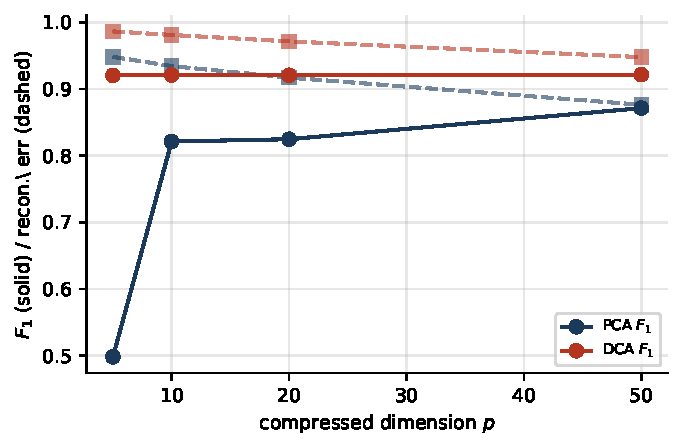
\includegraphics[width=\linewidth]{figs/compressive.pdf}
\captionof{figure}{Detection $F_1$ and reconstruction error vs dimension.}\label{fig:comp}\end{minipage}

\subsection{Coverage synthesis}
Table~\ref{tab:cov} consolidates which mechanism addresses which threat on the IDS.
\begin{table}[htbp]\centering\caption{Threat--defence coverage (\cmark{} stops, \pmark{} partial).}\label{tab:cov}
\begin{tabular}{p{3.5cm}p{3.0cm}cp{4.4cm}}
\toprule
Threat & Mechanism & Stops? & Note \\
\midrule
Backdoor poisoning (integrity) & DP-SGD training & \pmark & Clipping+noise limit poison influence; measured by ASR-vs-$\varepsilon$ \\
Membership inference & DP-SGD training & \cmark & Bounds per-window influence \\
Membership inference & Output modification & \pmark & Removes the confidence signal \\
Telemetry disclosure at collection & Local DP perturbation & \cmark & No trusted curator \\
Raw-window reconstruction & Compressive PCA/DCA & \cmark & Low-dim code discards raw signal \\
Frame re-identification & CAN-ID $k$-anonymity (analytical) & \pmark & Stream, not a classic table \\
\bottomrule
\end{tabular}
\end{table}

\subsection{Limitations and validity}
The mirror is a repackaged/relabelled copy, so the task is framed as binary
normal-vs-attack; attack captures are wholly attacked, so the class balance is a
sampling choice; and the honest detector is near-perfect because these CAN attacks
are statistically blunt -- which is the point (a near-perfect guard is silently
defeated), not a flaw. None of these change the direction of the results.

% ===== 5 =====
\section{Conclusions and Final Documentation}\label{sec:concl}
A trigger-based backdoor turns a near-perfect CAN intrusion detector into one that
passes real attacks on command, while staying invisible on clean traffic.
Differentially private training is the one mechanism that both protects the
training windows and attacks the backdoor's own mechanism; local DP and
compressive privacy protect the telemetry at a measured utility cost. All results
are reproducible from \texttt{IA2/scripts/run\_all.py} (full codebase at
\url{https://github.com/aish475/MLCS_IA}); a companion IEEE-format manuscript
accompanies this report.

\bibliographystyle{plainnat}
\bibliography{refs}
\end{document}
